\subsection{研究背景}
容貌焦虑已成为现代社会一个不可忽视的心理健康问题,尤其在年轻群体中表现得尤为突出。
随着科技的进步和社交媒体的普及,人们对外貌的关注度日益增加。
这种焦虑不仅影响个人的心理健康,还可能对他们的社交、工作和生活产生负面影响。

近年来,多项研究调查揭示了容貌焦虑的普遍性。
例如,2021年中青校媒面向全国2063名高校学生进行的容貌焦虑话题调查显示,59.03\%的大学生存在一定程度的容貌焦虑。
这一数据表明,容貌焦虑已经成为大学生群体中一个值得关注的现象。
此外,社交媒体和互联网技术的发展,使得``标准美''的形象被广泛传播和推崇,进一步加剧了年轻人的外貌压力。

容貌焦虑的形成原因是多方面的。
主观心理因素如自卑、敏感和攀比心理是引发容貌焦虑的重要原因。
客观环境因素同样对容貌焦虑的产生起到了推波助澜的作用。社会规范和大众传媒所构建的``大众审美''标准,对个体产生了深远的影响。
职场中的``颜值经济''现象也加剧了容貌焦虑,一些行业和岗位对外貌有着较高的要求,使得外貌成为了评价个人能力和价值的一个标准。

容貌焦虑的研究不仅有助于深入了解这一现象的成因和影响,还能为个体提供有效的应对策略,帮助他们建立正确的自我认知和健康的审美观念。通过心理健康教育和社会支持,可以减轻容貌焦虑对年轻人的负面影响,促进他们的心理健康和全面发展。

\subsection{研究现状}
\subsubsection{陈雪莹}
陈雪莹采用问卷调查法和统计分析法,对大学生群体使用抖音短视频平台引发的容貌焦虑加速现象进行分析,发现理想美内化在抖音使用强度与容貌焦虑的影响路径中发挥中介作用,上行社会比较发挥调节作用。
并据此提出减少大学生容貌焦虑的有效建议,以纠正当前抖音使用对大学生群体产生的审美观念扭曲问题。\autocite{__2022-3}

但是该论文存在局限性:研究对象仅局限于抖音用户中的大学生,样本具有一定的局限性,可能无法完全代表所有大学生群体。此外,对于容貌焦虑的测量和评估可能存在一定的主观性。


\subsubsection{祝旭冉和尹升志}
祝旭冉和尹升志采用量表设计、问卷发放、深度访谈,提出了
容貌焦虑的诱因:引起大学生容貌焦虑的具体原因有身材不好、单眼皮、脸上有痣、脱发等。
大学生群体在容貌焦虑的认知、态度、行为3个方面之间极易出现失衡现象。
其中心理原因、他人评价和审美观念的普及这三点对于容貌焦虑的产生有很大影响。\autocite{__2023}


\subsubsection{李升和李敏}
李升和李敏分析了容貌焦虑的成因和对应的解决方法:不仅需要从个体层面加强青年心理健康教育和服务,使其形成自尊自信、
理性平和、积极向上的良好心理素质,还需要更多从社会层面关注青年女性``容貌焦虑''的形成机制及结果,通过对社会性别规范更为 面的引导与改善,
在社会层面培育起积极正向的关于 身体的社会价值观与开放包容的审美文化。
同时需要持续优化青年群体的文化环境,构建更为丰富的美育氛围,媒体和网络媒介的内容与传播需有益于青年群体的健康成长,避免消费社会中的身体商品化消费意 识形态侵蚀社会舆论,以此推进在社会中形成整体 性、全面性、积极性的美感文化。\autocite{__2022-2}

还有很多关于分析网络对于青少年容貌焦虑形成的文献\autocite{_sisi_2024}。

\subsubsection{局限性}
这些研究都未深入研究大学生产生容貌焦虑的过程中所受到的诸如社会规训、美容美体广告、新时期一些新思潮在网络上的广泛传播等具体因素的影响。

\subsection{研究目的及意义}

\subsubsection{个体角度}
在个体身心健康和时间管理层面,我们小组希望可以通过此次研究,引导有容貌焦虑的人群悦纳自己,
乐观生活,帮助他们建立包容的、多元的审美价值体系,不被社会价值体系所裹挟,从心出发做自己。

\subsubsection{社会群体}
在美的定义和标准多元化层面,我们小组希望可以通过研究让人们不再为社会审美所束缚,
让``审美多元化''真正深入人们心中,从而对社会平稳运行产生一定积极影响。

\subsection{概念界定}
容貌焦虑是指在放大颜值作用的环境下,很多人对于自己的外貌不够自信,从而产生出自卑、痛苦的心理病症。

容貌焦虑者本身没有容貌绝对缺陷,但总对自身的容貌产生自卑和不满情绪。

而容貌焦虑的具体表现分为三个方面,具体如
图(\ref{pic:juti})所示
\begin{figure}[htbp]
    \centering
    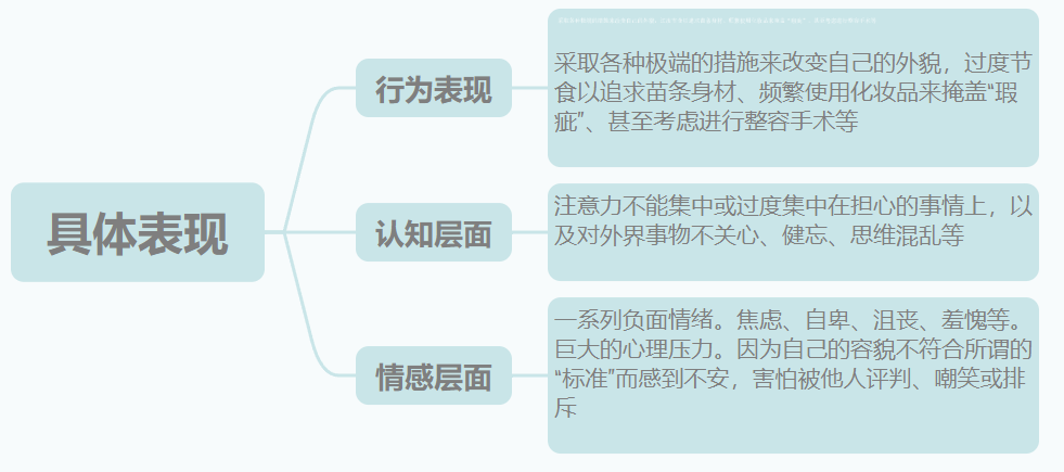
\includegraphics[width=0.7\textwidth]{具体表现.png}
    \caption{容貌焦虑的具体表现}
    \label{pic:juti}
\end{figure}


